\documentclass{article}
\usepackage{mhchem} % Package for chemical equation typesetting
\usepackage{siunitx} % Provides the \SI{}{} command for typesetting SI units
\usepackage{graphicx} % Required for the inclusion of images
\setlength\parindent{0pt} % Removes all indentation from paragraphs
\renewcommand{\labelenumi}{\alph{enumi}.} % Make numbering in the enumerate environment by letter rather than number (e.g. section 6)

\title{Determination of the Atomic \\ Weight of Magnesium \\ CHEM 101} % Title
\author{Luciano \textsc{Quercia}\\Simone \textsc{Rutigliano} }
\date{\today}


\begin{document}

\maketitle	

\begin{abstract}
Abstract text
\end{abstract}

%----------------------------------------------------------------------------------------
%	SECTION 1
%----------------------------------------------------------------------------------------

\section{Introduzione}

Il nostro progetto consiste nella realizzazione di un content-based recommender system che raccomandi film utilizzando dati provenienti dalla Linked Open Data Cloud al fine di poter aumentare l'efficienza del recommender system utilizzando informazioni aggiuntive inerenti un particolare film utilizzando differenti fonti.

\subsection{Linked Data}
L’interoperabilità è uno dei vantaggi più importanti del modello Open Data. I dati, se isolati, hanno poco valore; viceversa, il loro valore aumenta sensibilmente quando data set differenti, prodotti e pubblicati in modo indipendente da diversi soggetti, possono essere incrociati liberamente da terze parti. Questo è alla base del processo di creazione di valore aggiunto sui dati: le applicazioni. Le applicazioni, di valore sociale e/o economico, sfruttano quello che può essere visto come un grande database aperto e distribuito per offrire viste e servizi. L’interoperabilità è dunque un elemento chiave di uno degli aspetti più innovativi offerti dagli open data: l’uso dei dati in modi e per scopi “inattesi”, nuovi in quanto non previsti dai singoli enti e soggetti che pubblicano i “dati grezzi”.

Per consentire il riuso dei dati occorre poter combinare e mescolare liberamente i dataset. Occorre cioè collegare i dati tra loro, stabilendo un link diretto quando i dati (possibilmente provenienti da diverse sorgenti) si riferiscono a oggetti identici o comunque relazionati tra loro. Tale collegamento diretto si manifesta come la possibilità di “saltare” da un dataset all’altro, ad esempio quando si vuole accedere a dati (come i dettagli su una particolare entità) che non si posseggono al’interno.
Supponiamo per esempio di avere, da una parte, amministrazioni locali che pubblicano dati aperti relativi ai monumenti storici e agli hotel che si trovano nelle vicinanze di quei monumenti; dall’altra, Sovrintendenze ai Beni Culturali che pubblicano dati dettagliati sui monumenti, gli artisti e i periodi storici, e sui quadri esposti nei musei o nei palazzi.
Combinare i due dataset potrebbe essere di grande utilità, ad esempio per offrire un servizio personalizzato sugli itinerari in base agli interessi culturali specifici di un turista.
Per fare questo, se i dati non sono “collegati” (linked) occorre in qualche modo creare questi link, processando i dati a mano o attraverso algoritmi ad hoc. Questo processo può non essere banale e sicuramente è una barriera al riuso organico dei dati.

Nei cosiddetti Linked Data, questi collegamenti e relazioni tra le entità descritte nei dataset sono espliciti.
\subsection{Machine readable vs. machine linkable}
I linked data, per definizione, vengono espressi tramite Resource Description Framework (RDF). RDF non è propriamente un formato di dati, ma un “data model”, cioè un formalismo per rappresentare dati. Un dataset RDF può essere infatti serializzato in diversi formati (RDF/XML, N3, NTriple, etc.), ma il data model RDF possiede alcune caratteristiche che restano immutate, a prescindere dal formato che viene utilizzato.

In poche parole il modello RDF è costituito da triple, della forma soggetto-predicato-oggetto. Le triple possono condividere oggetto o soggetto così da formare un grafo.

\begin{figure}[htbp]
  \centering
  \includegraphics[width=.9\textwidth]
    {./images/triples1-crop}
\end{figure}

Questo insieme di triple RDF (o grafo) può essere espresso, allo scopo di essere scambiato tra applicazioni e pubblicato sul web, in vari formati di serializzazione.

Ad esempio in RDF/XML:
\lstset{ basicstyle=\LSTfont, columns=fullflexible, xleftmargin=5mm, framexleftmargin=5mm, numbers=left, stepnumber=1, breaklines=true, breakatwhitespace=false, numberstyle=\footnotesize, numbersep=5pt, tabsize=2, frame=lines, captionpos=b}
\begin{lstlisting}
<?xml version="1.0"?>
<rdf:RDF
    xmlns:ex="http://example.org/"
    xmlns:foaf="http://xmlns.com/foaf/0.1//"
    xmlns:rdf="http://www.w3.org/1999/02/22-rdf-syntax-ns#">
    <rdf:Description rdf:about="http://example.org/John">
        <foaf:knows>
            <rdf:Description rdf:about="http://example.org/Bob">
                <foaf:knows rdf:resource="http://example.org/Alice" />
            </rdf:Description>
        </foaf:knows>
    </rdf:Description>
</rdf:RDF>
\end{lstlisting}
La caratteristica più importante di tale modello, che si sposa con la visione Linked Data, è usare Uniform Resource Identifier (URI).



\section{Related Works}
\label{relatedworks}

Abbiamo affrontato lo stesso problema \citet{mirizzilinked} in un contesto differente.

Abbiamo implementato anche le formule per il calcolo della distanza contenute in \citet{passant2010measuring} 
per poterle confrontare con le nostre

\section{Misure}
\label{Measures}

\subsection{Distanze}

Il nostro recommender system è stato testato su quattro diverse misure di distanza.
Le prime due sono descritte in \citet{passant2010measuring}, le altre due è stata realizzata \emph{ex novo} e rappresentano una nuova visione pesata delle precedenti.


\subsubsection{Passant Direct}
\label{PassantD}
La distanza diretta. Indica il numero di archi diretti che collegano i film $a$ e $b$. Tenendo conto che il grafo preso in considerazione è orientato, vanno presi gli archi in entrambe le direzioni.

In maniera formale, definita $$C_{d}(f_a,f_b) = \left\vert \left\{ e \in Edges \  | \  (f_a \xrightarrow{~e~} f_b ) \right\} \right\vert$$ la formula della distanza completa sarà quindi:

%\begin{figure}[htbp]
%  \centering
%    \label{LDSD}
%    \begin{equation}
%        P_{d}(r_{a},r_{b}) = \frac{1} {1+C_{d}(n,r_{a},r_{b})+C_{d}(n,r_{b},r_{a})}
%    \end{equation}
%      \caption{LDSD Distance}
%      \label{LDSD1}
%\end{figure}

    \begin{equation}
        P_{d}(f_{a},f_{b}) = \frac{1} {1+C_{d}(f_{a},f_{b})+C_{d}(f_{b},f_{a})}
    \end{equation}

\subsubsection{Passant Combinated}
\label{PassantC}

La distanza combinata compone la precedente distanza diretta con una misura
(PassantI) che prende in considerazione i percorsi che uniscono due film
attraverso un film in comune.

PassantI restituisce un valore che indica il numero di archi che
mettono in relazione i due film attraverso dei film in comune.

Formalmente, definiti:
$$C_{io}(f_a,f_b) = \left\vert \left\{ f \  | \  (f_a \xrightarrow{~e~} f ) \wedge (f_b \xrightarrow{~e~} f) \right\} \right\vert$$
$$C_{ii}(f_a,f_b) = \left\vert \left\{ f \  | \  ( f \xrightarrow{~e~} f_a ) \wedge ( f \xrightarrow{~e~} f_b) \right\} \right\vert$$
$$\text{con} \ e \in Edges  , \qquad f_a,f_b,f \in Films $$

la formula indiretta di Passant è:
    \begin{equation}
        P_i(f_{a},f_{b}) = \frac{1} {1+C_{io}(f_{a},f_{b})+C_{ii}(f_{a},f_{b})}
    \end{equation}

La formula combinata sarà:

    \begin{equation}
P_{c}(f_{a},f_{b}) = \frac{1} {1+C_{d}(f_{a},f_{b})+C_{d}(f_{b},f_{a})+C_{io}(f_{a},f_{b})+C_{ii}(f_{a},f_{b})}
    \end{equation}


\subsubsection{Passant Direct Weighted}
\label{PassantDW}
La distanza diretta pesata, realizzata da noi, è una variazione della distanza diretta descritta in \ref{PassantD} che, invece che contare il numero di archi, somma i pesi di ciascun arco.

In maniera formale:

\begin{equation}
P_{dw}(f_a,f_b) = \sum\limits_{e \in ED}^{}{w(e)}
\end{equation}

con~~$ \qquad ED_{f_a,f_b} = \left\{ e \in Edges \quad\big\vert\quad f_a \xrightarrow{~e~} f_b \right\}$\footnote{Ricordando che nel nostro caso, trattandosi di un multigrafo, possono esserci più archi a collegare $f_a$ e $f_b$}

\subsubsection{Passant Combinated Weighted}
La distanza combinata pesata utilizza la precedente diretta pesata
\ref{PassantDW} insieme con la distanza che prende in considerazione i percorsi che uniscono due film attraverso un film in comune.

La distanza combinata, quindi, prende in considerazione sia gli archi diretti che gli archi indiretti (quelli che uniscono i film $a$ e $b$ passando da un film $c$ comune, come descritto in \ref{PassantC}). In questo caso, tuttavia, tutti gli archi sono pesati e la distanza corrisponde ad una sommatoria di pesi. In maniera formale, dati
$$EIO_{f_a,f_b} = \left\{ (e_1, e_2) \in Edges \quad\big\vert\quad f_a \xrightarrow{e_1} f_c \wedge f_b \xrightarrow{e_2} f_c \wedge label(e_1)=label(e_2) \right\}$$
$$EII_{f_a,f_b} = \left\{ p \in Paths \quad\big\vert\quad f_a \xrightarrow{e} f_c \wedge f_b \xrightarrow{e} f_c \right\}$$

\begin{equation}
CW_{io}(f_a,f_b) = \sum\limits_{(e_1,e_2) \in EIO_{f_a,f_b}^{}}^{}{w(e_1)*w(e_2)}
\end{equation}
\begin{equation}
CW_{ii}(f_a,f_b) = \sum\limits_{(e_1,e_2) \in EII_{f_a,f_b}^{}}^{}{w(e_1)*w(e_2)}
\end{equation}


\begin{equation}
P_{cw}(f_a,f_b) = \sum\limits_{(e_1,e_2) \in EII_{f_a,f_b}^{}}^{}{w(e_1)*w(e_2)}
\end{equation}

\subsection{Profili}

\subsubsection{Simple}
Il profilo coincide con l'insieme dei film valutati positivamente (4 e 5 considerati in egual misura)

\subsubsection{Simple Negative}

I film valutati 4 e 5 sono nell'insieme dei positivi. I film valutati 1 e 2 sono nell'insieme dei negativi.


\subsubsection{Voted Nostra}


Il profilo è l'insieme dei film visti, pesati secondo la formula:
votazioni dei film visti - voto medio dei film.

\subsubsection{Voted Musto}

Il profilo è l'insieme dei film visti, pesati secondo la formula:
Voto massimo + 1 - voto del film visto.


\section{Progetto}
\label{project}

Il progetto è composto da 5 package:
\begin{itemize}
\item\emph{graph}
\item\emph{distances}
\item\emph{profile}
\item\emph{recommendation}
\item\emph{movielens\_exp}
\end{itemize}

\subsection{Package graph}
Nella parte iniziale del progetto verranno eseguiti dei metodi presenti nella classi situate all'interno del package \emph{graph}, i cui scopi saranno quelli di:
\begin{itemize}
\item Salvare all'interno di un grafo i film presenti nel db di movielens\footnote{\url{http://www.grouplens.org/node/73}};
\item A partire dal grafo creato in precedenza, si va a creare un nuovo grafo in cui ogni vertice rappresenta un film, mentre ogni arco rappresenta un possibile collegamento che intercorre tra due film attraverso un qualunque tipo di risorsa quale ad esempio un particolare attore facente parte del casting di entrambi i film presi in considerazione.
\end{itemize}
\subsubsection{Graph}
Al fine di soddisfare il primo obiettivo, il primo metodo che verrà eseguito, sarà il metodo \emph{load}, il quale andrà a caricare da file binario serializzato il grafo da utilizzare all'interno del progetto; in caso contrario, quindi qualora il file non fosse presente, compito del metodo, sarà quello di creare la struttura dati graph che verrà utilizzata all'interno del progetto; per fare ciò, all'interno del metodo \emph{load} sarà presente il metodo \emph{createfromQuery}, il quale per ogni film presente all'interno del file di configurazione\footnote{\emph{ListFilms.txt} contiene ID di movielens, nome e URI di DBpedia di ogni film}, andrà innanzitutto ad inserire tali film come vertici del grafo e successivamente, per ogni proprietà presente anch'essa nel relativo file di configurazione, andrà a recuperare le risorse a cui sono collegate le risorse sorgenti con le varie proprietà; per fare ciò sarà presente il metodo \emph{querySPARQL}, il quale andrà ad eseguire la vera e propria query SPARQL all'endpoint di DBPedia\footnote{\url{http://dbpedia.org/sparql}} usando come soggetto l'URI della risorsa e come proprietà l'URI della proprietà, entrambi passati come parametro alla funzione stessa. Qualora il resultset della query dovesse essere positivo, quindi ci sono dei risultati, verranno creati all'interno del grafo sia i vertici contenenti le risorse ottenute dalla query, sia gli archi che ne permettano il cammino tra le due risorse; inoltre tale arco non sarà uniforme, ma sarà pesato in base al valore di pesatura di quella proprietà presente sempre all'interno del file di configurazione delle proprietà 
Una volta ottenute tutte queste informazioni e popolato l'intero grafo sia di archi, quindi predicati che mettano in relazione le risorse quale ad esempio director,writer,music composer e cosi via, che di vertici, quindi risorse quali film,attori,case produttrici,registi,ecc; tale grafo verrà serializzato al fine di ottimizzare future esecuzioni del progetto. Il grafo creato in questi passi sarà un tipo di multigrafo sparso e non direzionato.
Lo stesso package conterrà anche il metodo \emph{update} il quale avrà il compito di aggiornare i pesi dei vari archi senza necessariamente andarlo a ricreare da zero.

\subsubsection{FilmGraph}
Per quanto riguarda il secondo obiettivo,all'interno della classe \textsc{FilmGraph} sarà presente sempre un metodo \emph{load} il quale scopo è sempre quello di caricare qualora dovesse essere presente il file seriale dell'oggetto FilmGraph al fine di ottimizzare il calcolo computazionale del sistema; qualora non dovesse essere presente, si passa alla fase di creazione del nuovo grafo, in particolare un multigrafo sparso direzionato, partendo dal multigrafo sparso non direzionato creato in precedenza.
Per fare ciò, il nuovo grafo avrà come vertici solo ed esclusivamente i film di movielens presenti nel file di configurazione, mentre come archi tutti i possibili percorsi di lunghezza 2 necessari ad arrivare dal film sorgente al film destinatario, ad esempio: Partendo dal grafo delle risorse cosi composto 
\begin{figure}[H]
	\begin{tikzpicture}
	[lineDecorate/.style={-,thick},%
	  actor/.style={shape=circle,inner sep=3pt,draw, thick},
	  film/.style={shape=diamond,inner sep=4pt,draw,thick, fill=blue!15}]
	
	%% nodes or vertices
	\foreach \nodename/\x/\y/\direction/\navigate in {
	  $Django Unchained$/1/3/left/west, $Inglourious Basterds$/3/3/right/east, $Titanic$/1/1/below/south}
	{
	  \node (\nodename) at (\x,\y) [film] {};
	  \node [\direction] at (\nodename.\navigate) {\footnotesize$\nodename$};
	}
	
	\foreach \nodename/\x/\y/\direction/\navigate in {
	  $Quentin Tarantino$/2/4/above/north, $Leonardo Di caprio$/1/2/left/west, $Christoph Waltz$/3/2/right/east}
	{
	  \node (\nodename) at (\x,\y) [actor] {};
	  \node [\direction] at (\nodename.\navigate) {\footnotesize$\nodename$};
	}
	
	%% edges or lines
	\path
	\foreach \startnode/\endnode in {$Django Unchained$/$Leonardo Di caprio$, $Django Unchained$/$Christoph Waltz$, $Inglourious Basterds$/$Christoph Waltz$, $Leonardo Di caprio$/$Titanic$}
	{
	  (\startnode) edge[lineDecorate,director edge] node {} (\endnode)
	}
	
	\foreach \startnode/\endnode in {$Django Unchained$/$Quentin Tarantino$,$Quentin Tarantino$/$Inglourious Basterds$}
	{
	  (\startnode) edge[lineDecorate,bend left,actor edge] node {} (\endnode)
	}
	
	\foreach \startnode/\endnode in {$Quentin Tarantino$/$Django Unchained$, $Inglourious Basterds$/$Quentin Tarantino$}
	{
	  (\startnode) edge[lineDecorate,bend left,director edge] node {} (\endnode)
	};
	
	\end{tikzpicture}

	\begin{tabular}{l l}
	 \begin{tikzpicture}[film/.style={shape=diamond,inner sep=3pt,draw,thick, fill=blue!15}]
	  \node (a) at (6,3) [film] {};
	  \node [right] at (a.west) {\footnotesize};
	 \end{tikzpicture}
	 & \emph{Film} \\
		
	 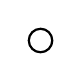
\begin{tikzpicture}[actor/.style={shape=circle,inner sep=3pt,draw, thick}]
	  \node (a) at (9,3) [actor] {};
	  \node [right] at (a.west) {\footnotesize};
	 \end{tikzpicture}
	 & \emph{Resource} \\	
		
	 \color{red}--- & \emph{Edge director} \\
	 \color{blue}--- & \emph{Edge actor} \\
	\end{tabular}	
\end{figure}
Si ottiene un nuovo multigrafo sparso direzionato di questo tipo:
\begin{figure}[H]
	\centering
	\begin{tikzpicture}
	[lineDecorate/.style={-,thick},%
	  film/.style={shape=diamond,inner sep=4pt,draw,thick, fill=blue!15}]
	
	%% nodes or vertices
	\foreach \nodename/\x/\y/\direction/\navigate in {
	  $Django Unchained$/0/4/left/west, $Inglourious Basterds$/4/4/right/east, $Titanic$/0/1/below/south}
	{
	  \node (\nodename) at (\x,\y) [film] {};
	  \node [\direction] at (\nodename.\navigate) {\small$\nodename$};
	}
	  \node ($actor Di Caprio actor$) at (0,2) {\color{red}\scriptsize{actor Di Caprio actor}};
	
	%% edges or lines
	\path
	\foreach \startnode/\endnode in {$Django Unchained$/$actor Di Caprio actor$,$actor Di Caprio actor$/$Titanic$}
	{
	  (\startnode) edge[lineDecorate,actor edge] node[] {} (\endnode)
	}
	
	\foreach \startnode/\endnode in {$Django Unchained$/$Inglourious Basterds$}
	{
	  (\startnode) edge[lineDecorate,bend left,actor edge] node[auto] {\scriptsize{actor Tarantino actor}} (\endnode)
	}
	
	\foreach \startnode/\endnode in {$Inglourious Basterds$/$Django Unchained$}
	{
	  (\startnode) edge[lineDecorate,bend left,director edge] node[auto] {\scriptsize{director Tarantino director}} (\endnode)
	};
	
	\end{tikzpicture}
\end{figure}

\begin{figure}[H]
	\includegraphics[width=\textwidth]{./images/Diagrams/graph.png}
	\caption{\emph{Class diagram: Package graph}}
\end{figure}

\subsection{Package distance}
\label{Package distance}
Il compito principale di questo package è quello di creare sia tutte le distanze di Passant (verranno definite nel dettaglio nei paragrafi \ref{PassantD} e \ref{PassantC}), sia le distanze da noi implementate (\ref{PassantDW} e \ref{PassantCW}). Per fare ciò, inizialmente verrà creato un hashmap tra la tipologia di distanza (PassantD, PassantC, PassantDW, ...) e l'oggetto \emph{distance} della relativa distanza; tale oggetto conterrà al suo interno un ulteriore hashmap tra la coppia di film e la relativa distanza che intercorre tra essi. In particolare, il metodo invocherà la classe astratta \emph{Distance} la quale, a sua volta, andrà ad implementare la relativa classe specifica.

\begin{figure}[H]
	\advance\leftskip-3cm
	\includegraphics[width=1.45\textwidth]{./images/Diagrams/distance.png}
	\caption{\emph{Class diagram: Package distance}}
\end{figure}

\subsection{Package profile}
Tramite le classi presenti all'interno di questo package, sarà possibile implementare le due tipologie di profilo (pesato e non pesato)(verranno descritte in dettaglio nel paragrafo \ref{profili}). 

In particolare, con la classe \emph{ProfileNotWeighted} (estensione della classe \emph{Profile}), verranno create due collezioni di film nelle quali saranno presenti, in una i film votati positivamente, e nell'altra i film giudicati negativamente\footnote{I film presenti in entrambe le collezioni avranno peso uniforme.}; invece, con la classe \emph{ProfileWeighted}, anch'essa estensione della classe \emph{Profile}, si andrà a creare solo una collezione di film i quali avranno anche un attributo caratterizzante il peso del film in proporzione al voto dato, in particolare secondo la formula che verrà descritta nel paragrafo \ref{profili}. 
\begin{figure}[H]
	\includegraphics[width=\textwidth]{./images/Diagrams/profile.png}
	\caption{\emph{Class diagram: Package profile}}
\end{figure}

\subsection{Package recommendation}
Come dice il nome stesso, il compito di questo package consiste nella vera e propria fase di raccomandazione ad un utente partendo da una particolare configurazione. Per configurazione si intende definire innanzitutto ia tipologia di \emph{\textbf{distanza}} da utilizzare, poi quale tipo di profilo utente utilizzare (\emph{\textbf{pesato}} o \emph{\textbf{non pesato}}) e infine il numero \emph{\textbf{k}} di raccomandazioni da generare.

All'interno di questo package sono presenti essenzialmente due classi:
\begin{itemize}
\item \emph{Recommendation} 
\item \emph{Recommender}
\end{itemize} 
La prima ha lo scopo di definire la struttura dati che verrà restituita dalla raccomandazione; in particolar modo, restituirà la coppia Film-distanza, dove per \emph{Film} si intende la struttura dati contenente tutte le informazioni circa il film, quindi ID di movielens e URI di DBpedia a cui si riferisce; mentre per distanza si intende il valore numerico con precisione \emph{double} ottenuto dal calcolo delle distanze tra il film in questione e il film sorgente di riferimento.

La seconda classe invece, ha come obiettivo quello di effettuare la vera e propria raccomandazione, per fare ciò, si andrà a creare una struttura dati di tipo hashmap avente come primo parametro caratterizzante le diverse tipologie di distanze, mentre come secondo parametro un ulteriore hashmap aventi come parametro i diversi film e come secondo la lista di raccomandazioni partendo dal film utilizzato come parametro del secondo map e come distanza, il valore numerico ottenuto dal calcolo effettuato dal package distance definito precedentemente \ref{Package distance}. 

Graficamente la struttura dati può essere rappresentato in questo modo:

\begin{table}[H]
	\begin{tabular}{l | l | l | l }
	\emph{DISTANCE\_TYPE} & \emph{FILM\_SRC} & \emph{FILM\_DEST} & \emph{VAL\_DISTANCE} \\
	\toprule
		\multirow{6}{*}{PassantD} & \multirow{3}{*}{Film1} & Film2 & 0.9 \\
		&  & Film3 & 0.8 \\
		&  & Film4 & 0.7 \\ \cline{2-4}
		& \multirow{2}{*}{Film5} & Film6 & 0.95 \\ 
		& & Film7 & 0.8 \\
		& & Film8 & 0.7 \\ \bottomrule
		\multirow{6}{*}{PassantDW} & \multirow{3}{*}{Film1} & Film2 & 0.96 \\
		&  & Film4 & 0.91 \\ 
		&  & Film3 & 0.80 \\ \cline{2-4}
		& \multirow{2}{*}{Film5} & Film21 & 0.9 \\ 
		& & Film10 & 0.82 \\
		& & Film7 & 0.76 \\ \bottomrule
		... & ... & ... & ....
	\end{tabular}
\end{table}


\subsection{Package movielens\_exp}
Il package \emph{movielens\_exp} ha il compito di eseguire la vera e propria fase sperimentale del progetto; In base a quanto verrà definito in seguito nel protocollo sperimentale \ref{experiment},



innanzitutto viene eseguita la fase di splitting delle votazioni date da ogni utente ai vari film visionati allo scopo di creare i set di training e di test. Successivamente si passa alla creazione dei profili(\emph{pesato} e \emph{non pesato}) partendo dalle votazioni presenti all'interno del training set di ogni utente; infine nella parte finale della sperimentazione vengono calcolate le diverse tipologie di metriche descritte in \ref{metriche}.


\section{Sperimentazione}
\label{experiment}
\lipsum[0-1]
\subsection{Metriche}
\label{metriche}

Al fine di valutare la bontà del sistema creato abbiamo calcolato due tipologie di metriche:
\begin{itemize}
\item Precision
\item MRR
\end{itemize}
Per entrambe le tipologie sono stati presi in esame due punti di vista differenti (\emph{macroscopico} e \emph{microscopico}) ed inoltre, per ogni punto di vista, si è lavorato su due versioni differenti dello stesso dataset (\emph{epurato} e \emph{non epurato}).

\subsubsection{Precision}
In un processo di classificazione statistica, la \emph{precisione} per una classe è il numero di \emph{true positive} (il numero di oggetti etichettati correttamente come appartenenti alla classe) diviso il numero totale di elementi etichettati come appartenenti alla classe (la somma di \emph{true positive} e \emph{false positive}, che sono oggetti etichettati erroneamente come appartenenti alla classe).
Inoltre i termini true positive, true negative, false positive e false negative sono usati per confrontare la classificazione di un oggetto (l’etichetta di classe assegnata all’oggetto da un classificatore) con la corretta classificazione desiderata (la classe a cui in realtà appartiene l’oggetto).
\begin{equation*}
Precision =\frac{TP}{TP+FP}
\end{equation*}

\paragraph{MicroPrecision}
Nel calcolo della microprecisione, è necessario prendere in considerazione i singoli valori di true positive e di false positive di ogni singolo utente come descritto nella formula:
\begin{equation*}
MicroPrecision =\frac{\sum\limits_{u\in U}^{}TP_u}{\sum\limits_{u\in U}^{}TP_u+\sum\limits_{u\in U}^{}FP_u}
\end{equation*}

\paragraph{MacroPrecision}
Per quanto riguarda invece il calcolo della macroprecisione, si va a prendere in considerazione il valor medio delle singole precisioni definite a livello di utente. Formalmente può essere descritto secondo la formula:
\begin{equation*}
MacroPrecision =\frac{1}{|U|}\sum\limits_{u\in U}{Precision_u}
\end{equation*}

\subsubsection{MRR}
Il Mean Reciprocal Rank (MRR) è un indice statistico per valutare un processo che produce una lista di possibili risposte ad una interrogazione (query), ordinate per probabilità di correttezza.
\begin{equation*}
MRR = \frac{1}{|Q|}\sum_{i=1}^{Q}{\frac{1}{Rank_i}}
\end{equation*}

\paragraph{MicroMRR}
Nel calcolo della microMRR, è necessario prendere in considerazione i singoli ranking delle raccomandazioni fatte ad ogni utente come descritto nella formula:
\begin{equation*}
MicroMRR =\frac{\sum\limits_{i=1}^{|R|}{\frac{relevant(r_i)}{i}}}{\sum\limits_{i=1}^{|R|}{\frac{1}{i}}} \qquad relevant(r_i)=\begin{cases} 1 & \mbox{se }r_i\mbox{ è rilevante} \\ 0 & \mbox{altrimenti}
\end{cases}
\end{equation*}
\paragraph{MacroMRR}
Per quanto riguarda invece il calcolo della macroMRR, si va a prendere in considerazione il valor medio dei singoli MRR definiti a livello di utente. Formalmente può essere descritto secondo la formula:
\begin{equation*}
MacroMRR =\frac{1}{|U|}\sum_{u\in U}{MRR_u}
\end{equation*}




%----------------------------------------------------------------------------------------
%	BIBLIOGRAPHY
%----------------------------------------------------------------------------------------

\bibliographystyle{unsrt}

\bibliography{}

%----------------------------------------------------------------------------------------


\end{document}
